\section{Nivel Internacional}

\subsection{Antecedentes}
Tras la presentación de Bitcoin a partir del año 2008 \cite[]{alice_blockchain_2021}, como una solución al problema del doble gasto y un medio de pago puramente electrónico \cite[]{nakamoto_bitcoin_2008},
surgen copias de esta red con mejoras en cuanto a la escalabilidad y velocidad de transacciones. Cuando Ethereum hizo presencia  con
un enfoque diferente a Bitcoin, expande el uso de la Blockchain
con la incorporación de los smart contract \cite[]{ethereum_que_2020}.  %Estos son programas alojados en la Blockchain,
No tardaron en surgir otras  Blockchain similares a la de Ethereum, como EOS, 
NEO,  cada una de ellas  tiene su particularidad en sus objetivos, la manera de utilizarlos y sus protocolos.

Desde el surgimiento de Ethereum, se  desarrollaron aplicaciones que permiten
representar activos del mundo real, siendo estos: títulos de automotores, terrenos o propiedades inmuebles,
títulos académicos, u otros instrumentos que representen valores para las personas.
Desde el despliegue de Ethereum 1.0 en el año 2015 se crearon  aplicaciones de video juegos,
financieras, redes sociales, arte digital, entre otros. El mundo del  Blockchain es un mar de proyectos e innovaciones,
por ende se hará foco en el área de educación académica, especialmente
en la validación de certificados, títulos o documentaciones relacionadas a esta
área \cite[]{drescher_Blockchain_2017,cheng_Blockchain_2018}.



La tecnología Blockchain es muy utilizada en la administración pública en países como Estonia, 
donde tienen un modelo de gobierno electrónico que es la identidad digital, con ella los estonios tienen sus datos
que lo identifican electrónicamente, permite  acceder a servicios del pais y viajar por la Unión Europea.   
Tienen un sistema de ciudadanía e-Residenc que permite a los extranjeros  viajar a distintos países con su
registro digital. Usan sus documentos de identidad electrónica para editar y revisar 
documentos fiscales, solicitar beneficios de seguridad social y obtener servicios bancarios \cite[]{brys_cadena_2019}.

Estonia no es el único país que se beneficia de la tecnología  Blockchain. Ucrania usa un sistema 
eAuction 3.0, usado para el alquiler o ventas de bienes del Estado para combatir 
la corrupción y disminuir la burocracia.
En Suecia hay un proyecto que permite almacenar transacciones inmobiliarias
de forma que todas las contrapartes: los bancos, los agentes, los compradores y vendedores  pueden 
tener la oportunidad de seguir el proceso de la implementación del acuerdo después de su finalización.
También  Georgia, Grecia y Honduras aplican la tecnología
Blockchain \cite[]{brys_cadena_2019}.

\subsection{Tendencias}


 La Blockchain  es utilizado cada día  por distintos sectores para respaldar 
documentos, así también en casos de agricultura, y cada vez surgen nuevos proyectos \cite[]{Blockchain_federal_argentina_trazabilidad_nodate}. 

Actualmente el mundo del  Blockchain está en crecimiento con los proyectos relacionados a los 
criptoactivos, ya que la gran mayoría de los consumidores de esta tecnología lo usan para generar ingresos con las distintas manera que  ofrecen los proyectos.
Existen sistemas web que publican las criptoactivos con mayor relevancia según el relevamiento que realizan ellos, 
dos de estos sistemas web son CoinMarketCap y CoinGecko.

Durante el desarrollo de la investigación, mediante  la utilización de la herramienta Google Trends,
se compararon los términos de búsquedas  Bitcoin, Ethereum, Blockchain, DApp y Cryptocurrency, desde  la figura  \ref{img:google_trends} 
 se puede observar según la tabla de interés que genera la herramienta en un rango de 0 a 100, donde Bitcoin es el 
término de búsqueda más popular inclusive que la Blockchain y el término Cryptocurrency o Criptomoneda. En comparación con la búsqueda DApp esta última
no parece ser muy conocida.  


\begin{figure}[H]
    \centering
    {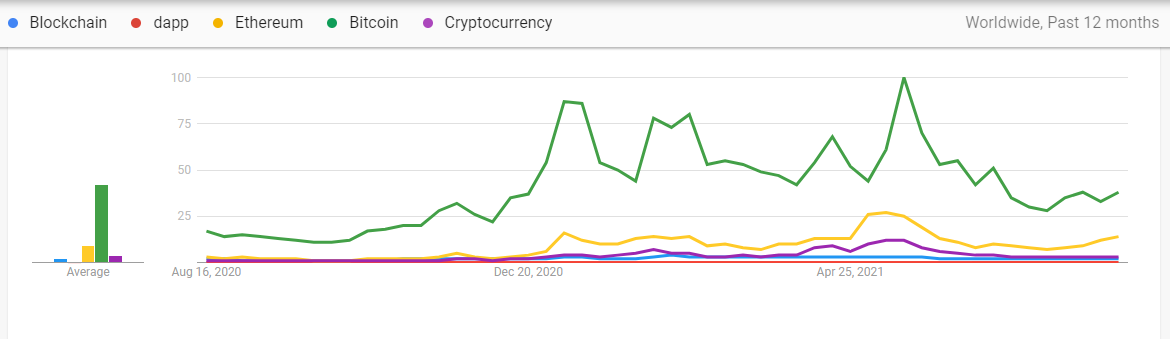
\includegraphics[scale=0.4]{google_trends.png}}
    \caption{Captura de pantalla de la  página Google Trends el dia 11/08/2021 } 
    \label{img:google_trends}
\end{figure}

En el mundo de la Blockchain las recientes tendencias fueron el uso de las Finanzas Descentralizadas (DeFi) y 
los Token No Fungibles (NFT). Las DeFi son muy consumidas en las últimas fechas por el retorno
de inversión que obtienen los usuarios a depositar sus criptoactivos. Y por el otro lado los NFTs
son unos criptoactivos que permiten representar la posesión de un elemento en particular, por ejemplo,
una obra de arte digital se puede comprar en el ecosistema de Blockchain, pero solo unos pocos usuarios serían dueños de ellos 
por en la escasez de ellos hacen que los NFT se han vendido a precios elevados \cite[]{brys_cadena_2019,cripto247_2021_2021}.

